\chapter{Security Challenges in Smart Constracts}
\markboth{Security Challenges in Smart Constracts}{}
\chaptauthors{Lucas Pelloni and Ile Cepilov}

\Kurzfassung{%
This is the abstract.
It fits pretty much on one page and is definitely not longer.}

\newpage

\minitoc %table of contents

\newpage
%http://blockgeeks.com/guides/what-is-blockchain-technology/
%http://www.investopedia.com/terms/b/blockchain.asp
%https://letstalkpayments.com/an-overview-of-blockchain-technology
% PWC: PAPER DA PRENDERE ASSOLUTAMENTE http://www.pwc.ch/en/2017/pdf/pwc_blockchain_opportunity_for_energy_producers_and_consumers_en.pdf


\section{Blockchain Technology}
\subsection{Definition of Blockchain}
A blockchain is like a distributed database which constantly keeps a list of transaction or records, that have ever been executed, called usually blocks. Every record contains a reference to its predecessor and a timestamp. \cite{wikipedia1}
Data in a record cannot be changed due to its design. This makes them tampering-proof and a very good source of trust for the near future. \cite{blockchain3}
The blockchain works and is maintained by the entire community, which verifies all records and acts like a node of a peer-to-peer network, making the need of a thirty part trust organisation useless. \cite{blockchain0}
\subsubsection{Source of Trust}
%http://www.investopedia.com/terms/b/blockchain.asp
Blockchain will become a global decentralised source of trust.
Everything that is centralized makes it easy to attack because it offers a single point of failure. 
(e.g. Firewall of a website). 
Application built with Bloch chain technlogy do not require  users to trust the developers with personal information or funds. 
\subsubsection{How does a Blockchain work?}
           \begin{figure}[ht]
         \begin{center}
         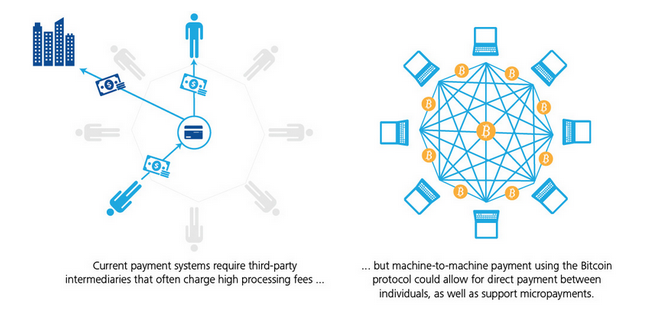
\includegraphics[scale=0.6]{Talk3/blockchain}
         \end{center}
         \caption{This is a pic FROM ILIA}
         \label{label}
       \end{figure}
   
%https://www2.deloitte.com/nl/nl/pages/innovatie/artikelen/blockchain-technology-9-benefits-and-7-challenges.html
\subsection{Benefits of Blockchain Technology}
Every technology that is centralized offers somewhere a point of failure which might be exploited by attackers and nowadays, banks are normally used by most people as a trusted middleman in order to make transaction.
Thanks to its decentralizations, blockchain will avoid the need of a trusted middleman to make transaction by connecting directly buyers and sellers\cite{blockchain4}
%TODO

%http://www.huffingtonpost.com/ameer-rosic-/5-blockchain-applications_b_13279010.html
\subsection{Blockchain applications}
The most famous application of blockchain is in online trades where it gets used for transfering a cryptovalue, bitcoins.\cite{blockchain9}
%TODO 


%https://www.shapingtomorrow.com/home/alert/665529-Future-of--Blockchain
%http://usblogs.pwc.com/emerging-technology/the-blockchain-problem-is-a-trust-problem/
\subsection{Future of Blockchain}
%TODO 

%https://www.taylorwessing.com/download/article-how-secure-is-block-chain.html
\subsection{Blockchain security}
%TODO 


\section{Smart Contract: Introduction}
\subsection{Smart Contract: a self-executing contractual agreements}
%definition founded here: https://www.youtube.com/watch?v=FkeLDPZ-v8g&t=134s
A Smart Contract is a computer protocol (or piece of software) that includes, simplifies and verifies the negotiating terms for the execution of a contract. They do not contain a formal contract clause but they usually simulate it.
Smart Contracts are encrypted and implemented as programs running on the nodes of a custom public blockchain network, which is not the same used for Bitcoins transactions. Thanks to their encryption, an external trusted authority is no longer needed and thanks to the redundancy of the blockchain across the network, there will not be any loss of data or integrity in case of a system failure.
If a new Smart Contract has to be added to the blockchain, the miners, which are the actual nodes of the peer to peer network, have first to validate its execution and only once it has been validated by the majority of them, it can be actually appended to the blockchain.
%https://bitsonblocks.net/2016/02/01/a-gentle-introduction-to-smart-contracts/%
\subsubsection{Traditional vs. Smart Contract}

\subsection{Ethereum: a public blockchain-based platform}
Ethereum is a platform for the publication and the execution of Smart Contracts. It is decentralized INSERIRE PAPER and executes the Smart Contracts as programmed from their creator.
It has a own cryptovalue called Ether which is used as payment for the execution of Smart Contracts.
At the 24th of April 2017, the value of the currency compared to Bitcoins corresponded to CONTINUA
Ethereum's contracts are written in Solidity, which is an objected-oriented language programming language, similar to Java, and it is exclusively designed for coding Smart Contracts.
The Smart Contracts are then compiled in the Ethereum virtual machine (EVM bytecode) and deployed finally on the Ethereum blockchain 

\subsection{Smart Contract's properties in Ethereum}
In this section we will have a look at the key components that can be found inside a Smart Contract.
A Smart Contract must always have a {\itshape contract address} 
%PAPER 633.pdf% asddd
which can be used to identify it. It may contain some amount of Ether (The virtual coin used in Ethereum) in its {\itshape balance} attribute.
\\It has a very important function which does not take any parameter at all, i.e. the so called {\itshape Fallback} function(). This function will be triggered by default when a contract is invoked by a transaction.
\\It is very important because, as we will see in the next sections, it has been exploited a lot in the most famous attacks.
\\Of course, some more informations have to be stored in it, like who the sender is, the amount of Ether that is sent to the contract and some more info for the transaction. All this data are saved in a variable {\textit msg.}
%http://www.coinfox.info/news/reviews/5195-ethereum-and-smart-contracts-in-depth
\\Now we would like to introduce the Gas system. The gas is used to express the cost of a computation done by the EVM, which in turn will be payed in the currency (Ether). Even though the actual currency may variate, the price of the network resources (Gas) stays constant.
\\The gas is divided in three main component, {\textit the Gas Cost, the Gas Price and the Gas Limit.}
\\The Gas Cost has a static value over time, whereas the Gas Price, measured in ether, changes accordingly to the cryptocurrency's fluctuation. But like we said before, the real cost of the Gas should remain the same, which means that an increase of the price of ether will have as a consequence a drop down of the Gas Price.
\\When somebody sends a transaction to invoke a contract, he has to specify hos much Gas he/she is willing to provide for its execution (Gas Limit). 
%To run a particular transaction or program (called “contract”), one has to pay an amount of Gas (called Gas %Fee) to miners. There is a list of fixed default fees for particular operations 




\subsubsection{Solidity: a typed JavaScript-like language}
TODO: CONTROLLARE LA VALIDITA 
As introduced in Ethereum, Solidity is a object-oriented programming language for writing smart contracts and it can be used on various blockchain even though it is used as the primary language on the Ethereum platform.
%https://en.wikipedia.org/wiki/Solidity
\\It was first proposed in August 2014 by Gavin Wood and developed later by the Ethereum project's Solidity team (CITA MEEENCHIA)

\section{Smart Contract attacks}

\subsection{DAO Attack}
\subsubsection{Attack description}
One of the most famous attack on Smart Contracts was the DAO Attack (Decentralised Autonomous Organisation).
%https://www.wired.com/2016/06/50-million-hack-just-showed-dao-human/
The DAO was a crowd-funding project which, like traditional mutual funds, allows investors or "members" to purchase shares and enjoy returns based on its performance.
On 17 June 2016, the attacker managed to steal 3.6 Milion Ether\footnote{Corresponding to USD 60 million} from the Ethereum's platform and putting them into a personal account. \\ %http://www.clydeco.com/insight/article/ethereums-dao-attack-smart-contracts-and-blockchain-face-their-first-big-te
Due to the strong impact of this attack to the Etherum platform, the value of the Ether currency drastically dropped from 20.5 USD to 11.20 USD (cita: %http://uk.businessinsider.com/dao-hacked-ethereum-crashing-in-value-tens-of-millions-allegedly-stolen-2016-6
). \\
We now consider only a streamlined version of the DAO attack, also called \textbf{SimpleDAO}, which is the first of the two known DAO attacks and has some common characteristics to the original one. The attack described below allows the hacker to siphon all the ether contained within the \textbf{SimpleDAO} Smart Contract.\cite{paper2} \\
The first thing the attacker has to do is to publish a \textbf{Mallory} Contract (as shown below): 
\begin{figure}[H]
\begin{center}
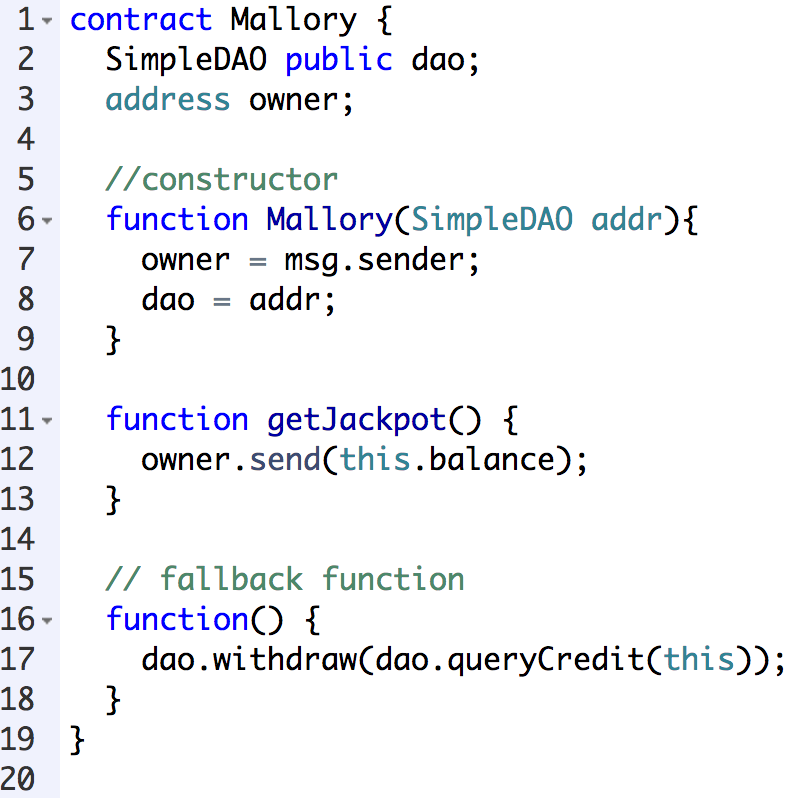
\includegraphics[scale=0.45]{Talk3/img/dao1}
\end{center}
\caption{Dao Attack: the Mallory contract}
\label{label}
\end{figure}
%https://github.com/chriseth/solidity-doc-test/blob/master/docs/frequently-asked-questions.rst
%http://solidity.readthedocs.io/en/latest/frequently-asked-questions.html
After publishing the contract, the hacker sends some Ether to Mallory and automatically invokes the Mallory Fallback\footnote{A Fallback is just a function without any name or parameter, which is called by default if some ether is sent to a contract. (cita) } (line 16, \textbf{Mallory}). \\
The \textbf{Mallory}'s fallback, in turn, calls the \textbf{withdraw} function written in the \textbf{SimpleDAO}\footnote{The whole Smart Contract's code is findable here: http://co2.unica.it/ethereum/attacks.html\#simpledao} contract (figure below), which is in charge of sending an amount of Ether to a specified public address. 
\begin{figure}[H]
\begin{center}
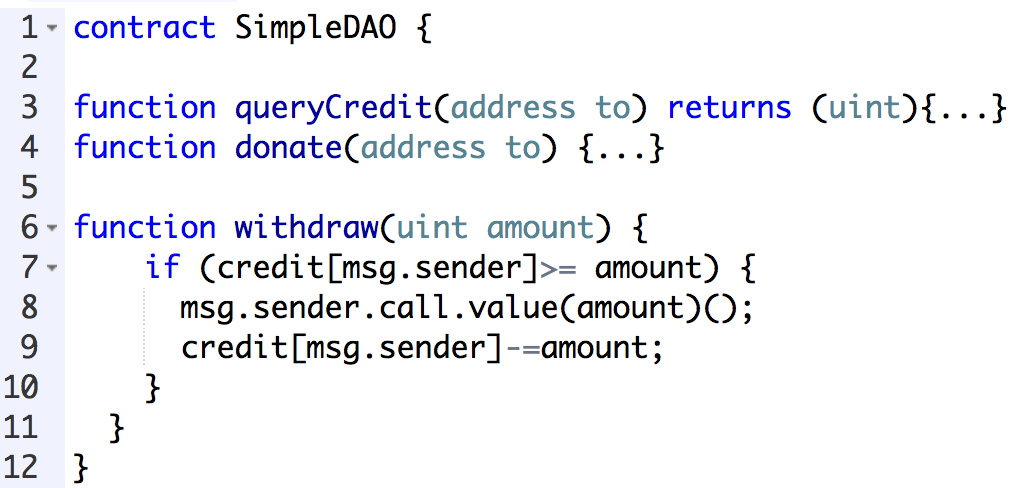
\includegraphics[scale=0.45]{Talk3/img/dao2}
\end{center}
\caption{Dao Attack: the SimpleDAO contract}
\label{label}
\end{figure}
Since the \textbf{withdraw} function of the \textbf{SimpleDAO} has been invoked by the \textbf{Mallory} fallback, it simply sends the Ether to Mallory (line 6, \textbf{SimpleDAO}). By sending the Ether to \textbf{Mallory}, the \textbf{Mallory}'s fallback gets invoked again. As a consequence, the \textbf{withdraw} function transfers the specified amount of Ether to \textbf{Mallory} for the second time. The flaw of this sequence of function calls resides at line 9 of the \textbf{SimpleDAO} contract, where the real amount of Ether stored within the contract gets never updated. 
This kind of loop goes on until one of the following conditions is satisfied: \\
\begin{enumerate}
%cita nella footnote: https://www.cryptocompare.com/coins/guides/what-is-the-gas-in-ethereum/
\item The gas is exhausted\footnote{Internal fee in Ethereum paid to the miners, proportional to their power computation}
\item Call Stack is full
\item Balance of DAO gets down to zero  
\end{enumerate}





\subsubsection{No solutions, only countermeasures}
Sadly, there was a lack of solutions for stopping this attack. The only possible choice was to suppress the attack and the community was faced with two of them.
\\A first choice was to do a {\textit Soft fork} which consisted in freezing the transaction that belonged to the attacker. But not the majority of the whole community agreed with it and more important, the transactions that were used by the attacker in order to move the stolen funds, would have ignored and not reverted and therefore the miners would not have been paid
\\Moreover, in doing so, a potential DOS attack would have been introduced. 
(cit:)
%https://steemit.com/crypto-news/@help-yourself/the-dao-soft-fork-solution-has-a-potential-dos-vector
Specifically, an attacker can flood the network with transactions that execute difficult computation, and end by performing an operation on the DAO contract. Miners running the soft fork would end up having to execute, and then subsequently discard, such contracts without collecting any fees.
\\Therefore a {\textit Soft fork} was proposed and approved on the 19th of July. Its intention was to put into a new refund Smart Contract all the ether taken by the attacker during the attack. The refund Smart Contract would have only one functions withdraw allowing the poor victims get back their stolen funds.
\subsection{MultiPlayer Attack}
\subsubsection{Attack description}
\subsubsection{Exploited vulnerability}
\subsubsection{Possible solution}

\subsection{Rubixi Attack}
\subsubsection{Attack description}
\subsubsection{Exploited vulnerability}
\subsubsection{Possible solution}


%sito originale: https://www.kingoftheether.com
%Post mordem: https://www.kingoftheether.com/postmortem.html
%source code: https://github.com/kieranelby/KingOfTheEtherThrone/blob/v0.4.0/contracts/KingOfTheEtherThrone.sol

\subsection{King of The Ether Throne}
The "King of the Ether" (or "King of the Ether Throne") is an Ethereum contract, stored on the blockchain, which implements a very simple game. cita: % https://www.kingoftheether.com 
The game's goal is to become the "King/Queen of the Ether". In order to make that possible, a player who wants to join the game has to pay an amount of Ether greater that the current claimprice. If the amount is greater, this player becomes the new King and a small fee has to be computed and paid to the old king. 
When a new King gets crowned, the claimprice is calculated and set as new prize of the game. The prize logically increases each time a new king is crowned \cite{paper2}. \\

\subsubsection{First Attack description}
For a proper explanation of this attack, consider the following \textbf{KotET} contract, which implements a simplified version of the original contract\footnote{the whole code can be found here: http://co2.unica.it/ethereum/attacks.html\#kotet}.   
\begin{figure}[H]
\begin{center}
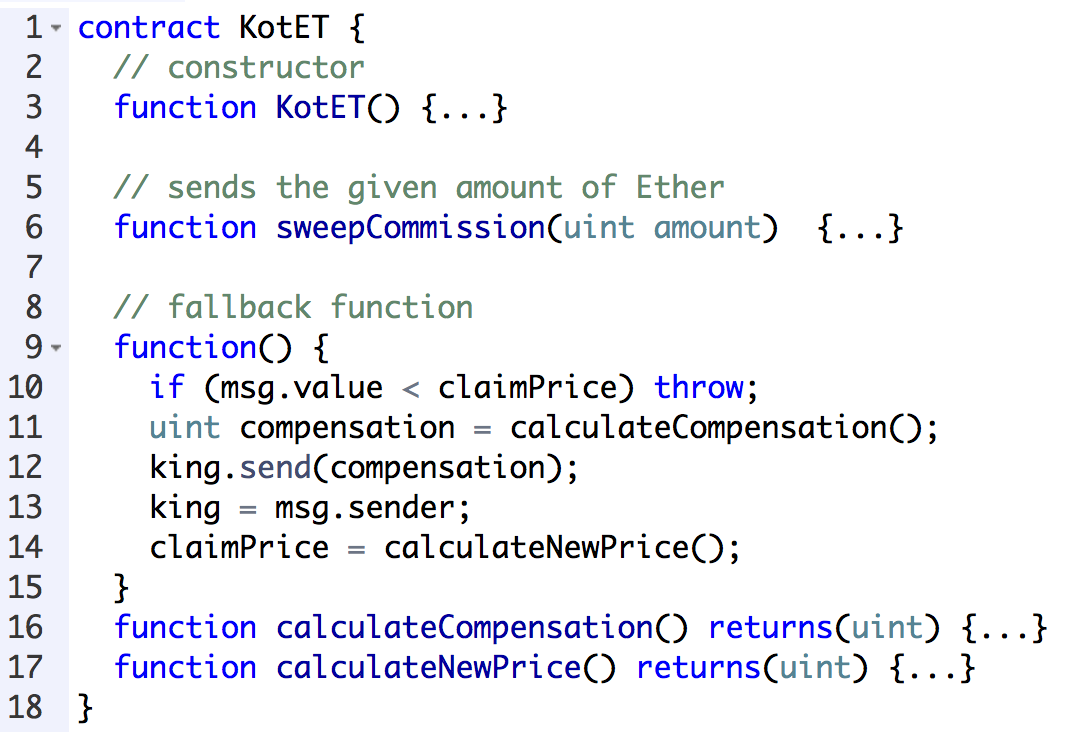
\includegraphics[scale=0.5]{Talk3/img/kot}
\end{center}
\caption{First KotET contract}
\label{label}
\end{figure}
Whenever a new player sends some Ether to the \textbf{KotET} contract, the fallback function gets invoked by default (line 9). The first "if-statement" inside the fallback function checks whether the sent Ether is greater that the current claimprice, otherwise an exception gets thrown and the whole transaction gets reverted. If the amount is enough, the compensation for the old king is computed and sent to him (line 11, 12). After that, the current player is crowned as new king and the new prize is calculated and stored inside the contract\cite{paper2}. \\
The flaw exploited in this attack resides at line 12. For this contract doesn't exist a control in the \textbf{return code} of the \textbf{send} function (cita) %da citare http://co2.unica.it/ethereum/attacks.html\#kotet 
and this may cause a lost of Ether.
If there would be someone, who wants to attack this contract, he could require much more gas for the \textbf{send} compensation function (which means, that his \textbf{fallback} function would be very expensive) (cita quello sopra). Indoing so, the function call at line 12 may fail and since there is no check in the return code (the \textbf{send} does not cause any exception) the compensation for the old king will thus remain by the contract, even in the case of a new crowned king. 
After that, the attacker could easily withdraw the compensation accumulated in the contract (via \textbf{sweepCommission}, at line 6).  

%cita questo: https://www.kingoftheether.com/contract-safety-checklist.html
\subsubsection{Possible solution}
The solution adapted by Ethereum to avoid future attacks is also known as the "failed sends" solution (cita). It consists of an attachment of a reasonable amount of gas with each transaction involving two or more parties (cita ancora). 
For example, if a miner would have a very expensive fallback function, an exception should be thrown and the whole transaction should be reverted. \\ For testing the accuracy of this solution Ethereum runned several functional tests\footnote{the simulated test cases described in th Ethereum on-chain report can be found here: https://github.com/kieranelby/KingOfTheEtherThrone/blob/v1.0/tests/onchain-test-report.md}, trying to cover the largest number of possible scenarios. 


\subsubsection{Second Attack description}
For making our explanation easier to understand, consider also in this case the following semplified \textbf{KotET} contract: 
\begin{figure}[H]
\begin{center}
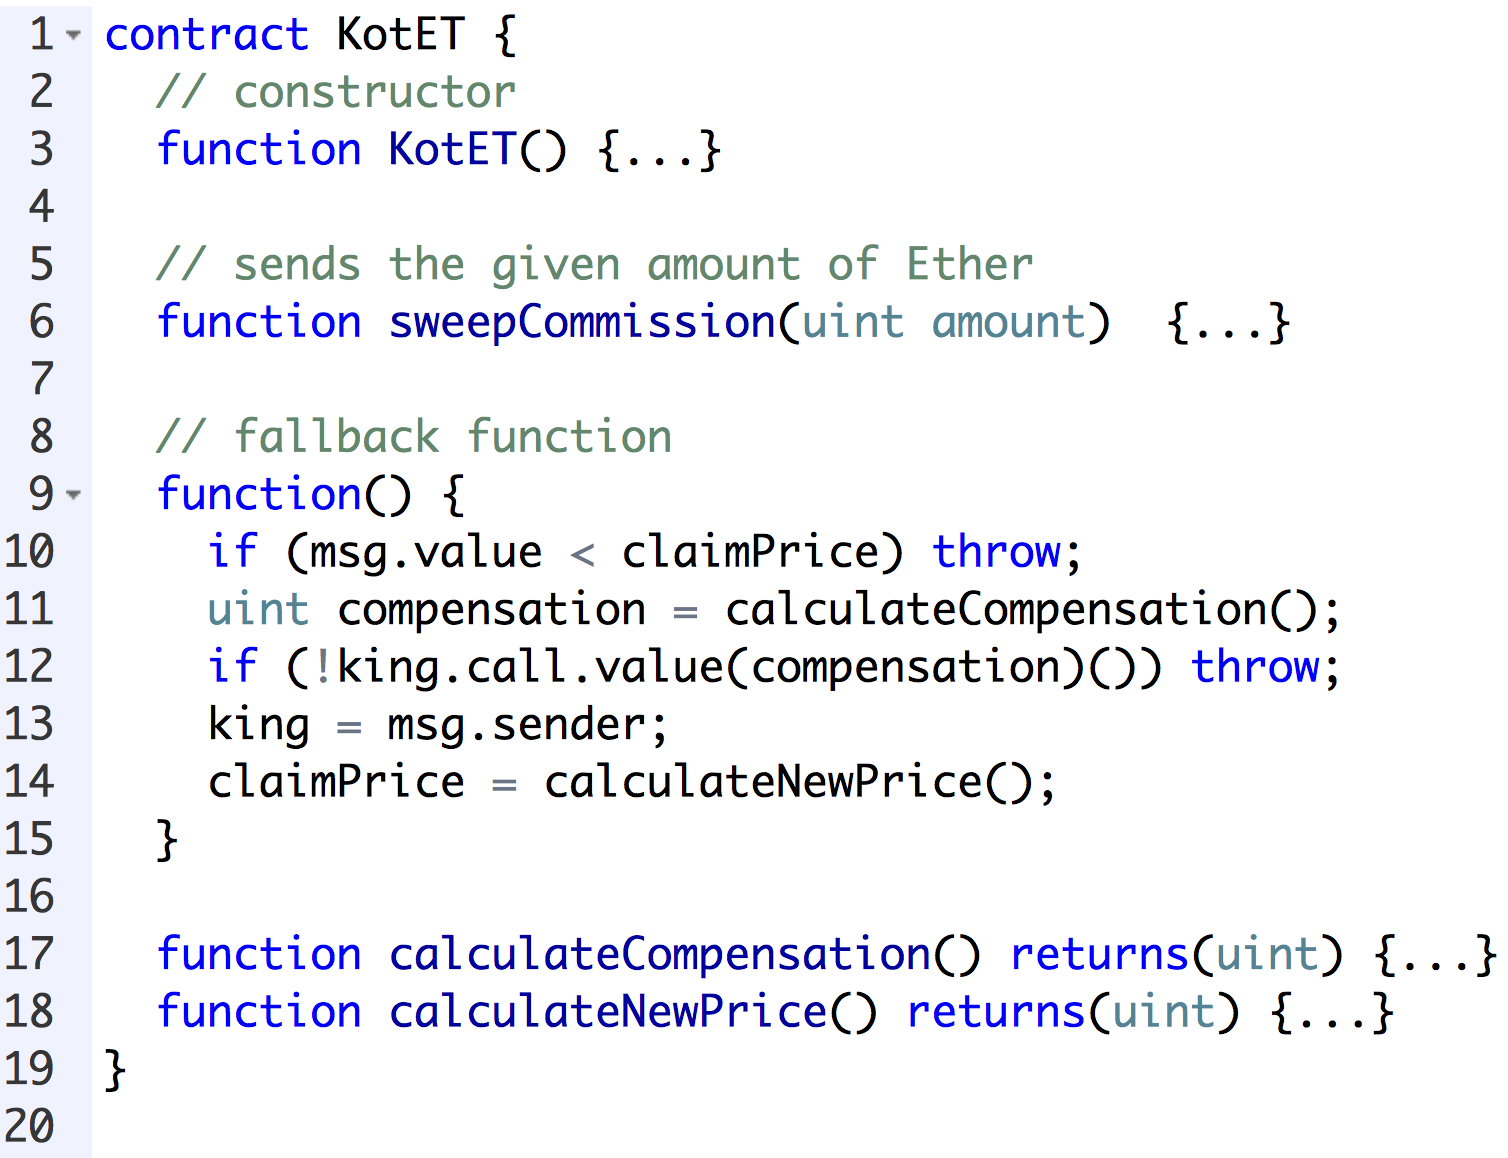
\includegraphics[scale=0.3]{Talk3/img/kot2}
\end{center}
\caption{Second KotET contract}
\label{label}
\end{figure}
As highlighted in the contract above, the only difference between the first KotET contract (mentioned in the paragraph above) and this contract resides in the \textbf{fallback function}, more specifically in the method with whom the compensation is sent to the old king. Indeed, the first contract implements a \textbf{send function}, while the second one uses a \textbf{call function} for transfering an amount of Ether. A \textbf{send} function is usually equipped with some gas\footnote{normally 2300 gas}, while a \textbf{call function} does not use any gas (cita). 
%difference between call/send: https://ethereum.stackexchange.com/questions/6470/send-vs-call-differences-and-when-to-use-and-when-not-to-use
Moreover, the second contract checks the return code of the \textbf{call} function and even though it should be more reliable that the first one, it can be also hacked. \\
Let's suppose that there would be someone, who wants to attack this contract publishing the following \textbf{Mallory} contract: 
\begin{figure}[H]
\begin{center}
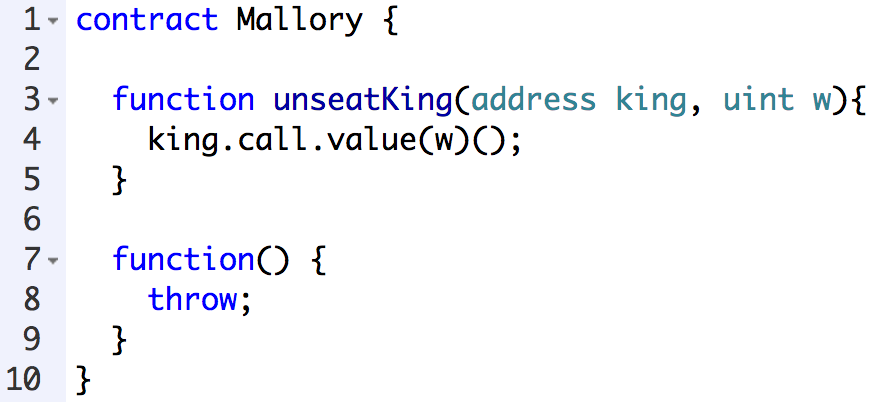
\includegraphics[scale=0.5]{Talk3/img/kot_mallory}
\end{center}
\caption{The KotET Mallory contract}
\label{label}
\end{figure}

This contract Mallory has a fallback, which just throws an exception. The hacker calls \textbf{unseatKing} with the right amount of Ether, so that Mallory becomes the new king. 
At this point, nobody else can get her crown, since every time \textbf{KotET} tries to send the compensation to Mallory, her fallback throws an exception, preventing the coronation to succeed. 

\subsubsection{Possible solution}

\subsection{Govern-Mental: First Attack}
Blablabla said asfbzasfubasbusauhfhu \cite{WinNT}.
\subsubsection{Attack description}
\subsubsection{Exploited vulnerability}
\subsubsection{Possible solution}

\subsection{Govern-Mental: Second Attack}
\subsubsection{Attack description}
\subsubsection{Exploited vulnerability}
\subsubsection{Possible solution}

%http://usblogs.pwc.com/emerging-technology/tag/blockchain/
%http://www.coindesk.com/blockchain-smart-contracts-looming-challenges/
\section{Security Challenges in Smart Contract}
\subsection{No guarantee of transaction execution}
\subsection{Slowness of Smart Contract}
\subsection{Code is slow}

\begin{thebibliography}{99}
\bibitem{ethereum1}\emph{Ethereum Homestead Release.} \url{https://www.ethereum.org} (last accessed March 2017)
\bibitem{wikipedia1}\emph{Blockchain} Wikipedia: \url{https://en.wikipedia.org/wiki/Blockchain} (last accessed February 2017)
\bibitem{blockchain1}\emph{Know More About Blockchain.} \url{https://letstalkpayments.com/an-overview-of-blockchain-technology/} (last accessed March 2017)
\bibitem{blockchain2}\emph{Blockchain Use Cases Part II.} \url{https://letstalkpayments.com/blockchain-use-cases-part-ii-non-financial-and-financial-use-cases/} (last accessed March 2017)


\bibitem{paper1}Loi Luu, Duc-Hiep Chu, Hrishi Olickel, Prateek Saxena, Aquinas Hobor: \emph{Making Smart Contracts Smarter.}. October 2016. \url{http://delivery.acm.org/10.1145/2980000/2978309/p254-luu.pdf?ip=195.176.96.218&id=2978309&acc=ACTIVE\%20SERVICE&key=FC66C24E42F07228\%2EA04051DB0C098788\%2E4D4702B0C3E38B35\%2E4D4702B0C3E38B35&CFID=926344688&CFTOKEN=88107312&__acm__=1492712435_d0f0d96ea04f8cf077c9b90253210778} (last accessed February 2016)

\bibitem{paper2}Atzei, Nicola and Bartoletti, Massimo and Cimoli, Tiziana: \emph{A survey of attacks on Ethereum smart contracts.} 2016. Cryptology ePrint Archive: Report 2016/1007, https://eprint. iacr. org/2016/1007 \url{https://eprint.iacr.org/2016/1007.pdf} (last accessed February 2017)

\bibitem{blockchain3}Investopedia: \emph{What is a Blockchain.} \url{http://www.investopedia.com/terms/b/blockchain.asp} (last accessed March 2017)

\bibitem{blockchain4}\emph{Blockchain technology: 9 benefits and 7 challenges.} \url{https://www2.deloitte.com/nl/nl/pages/innovatie/artikelen/blockchain-technology-9-benefits-and-7-challenges.html} (last accessed March 2017)

\bibitem{blockchain5}Hasse, von Perfall, Hillebrand, Smole, Lay, Charlet: \emph{Blockchain - an opportunity for energy producers and consumers?.}\url{http://www.pwc.ch/en/2017/pdf/pwc_blockchain_opportunity_for_energy_producers_and_consumers_en.pdf} (last accessed March 2017)

\bibitem{blockchain6}\emph{What is Blockchain Technology?.} \url{https://blockgeeks.com/guides/what-is-blockchain-technology/} (last accessed March 2017)
\bibitem{blockchain7}\emph{Know More About Blockchain.} \url{https://letstalkpayments.com/an-overview-of-blockchain-technology/} (last accessed April 2017)
\bibitem{blockchain8}\emph{Five Blockchain Applications That Are Shaping Your Future.}\url{http://www.huffingtonpost.com/ameer-rosic-/5-blockchain-applications_b_13279010.html} (last accessed March 2017)
\bibitem{blockchain9}\emph{Future of Blockchain.} \url{https://www.shapingtomorrow.com/home/alert/665529-Future-of--Blockchain} (last accessed February 2017)
\bibitem{blockchain10}\emph{The blockchain problem is a trust problem.}\url{http://usblogs.pwc.com/emerging-technology/the-blockchain-problem-is-a-trust-problem/} (last accessed February 2017)
\bibitem{blockchain11}\emph{How secure is blockchain?.} \url{https://www.taylorwessing.com/download/article-how-secure-is-block-chain.html} (last accessed March 2017)
\bibitem{SC1}\emph{Simple introduction to smart contracts on a blockchain.} \url{https://www.youtube.com/watch?v=FkeLDPZ-v8g&t=134s} (last accessed March 2017)
\bibitem{SC2}\emph{A gentle introduction to smart contracts.} \url{https://bitsonblocks.net/2016/02/01/a-gentle-introduction-to-smart-contracts/} (last accessed February 2017)
\bibitem{SC3}\emph{Blockchain Pros Debate Looming Challenges for Smart Contracts.} \url{http://www.coindesk.com/blockchain-smart-contracts-looming-challenges/} (last accessed April 2017)



\bibitem{blockchain0}Morabito: \emph{Blockchain Value System.} 2017. \url{http://www.springer.com/cda/content/document/cda_downloaddocument/9783319484778-c2.pdf?SGWID=0-0-45-1599947-p180347565} (last accessed March 2017)
\bibitem{SC5}\emph{title.}\url{url} (last accessed April 2017)
\bibitem{SC6}\emph{title.}\url{url} (last accessed April 2017)
\bibitem{SC7}\emph{title.}\url{url} (last accessed April 2017)
\bibitem{SC8}\emph{title.}\url{url} (last accessed April 2017)
\bibitem{SC9}\emph{title.}\url{url} (last accessed April 2017)
\bibitem{SC10}\emph{title.}\url{url} (last accessed April 2017)
\bibitem{SC11}\emph{title.}\url{url} (last accessed April 2017)
\bibitem{SC12}\emph{title.}\url{url} (last accessed April 2017)
\bibitem{SC13}\emph{title.}\url{url} (last accessed April 2017)









\end{thebibliography}
